% !TeX root = ../0_Manuscript.tex

%\begin{figure}[ht]
%    \centering
%    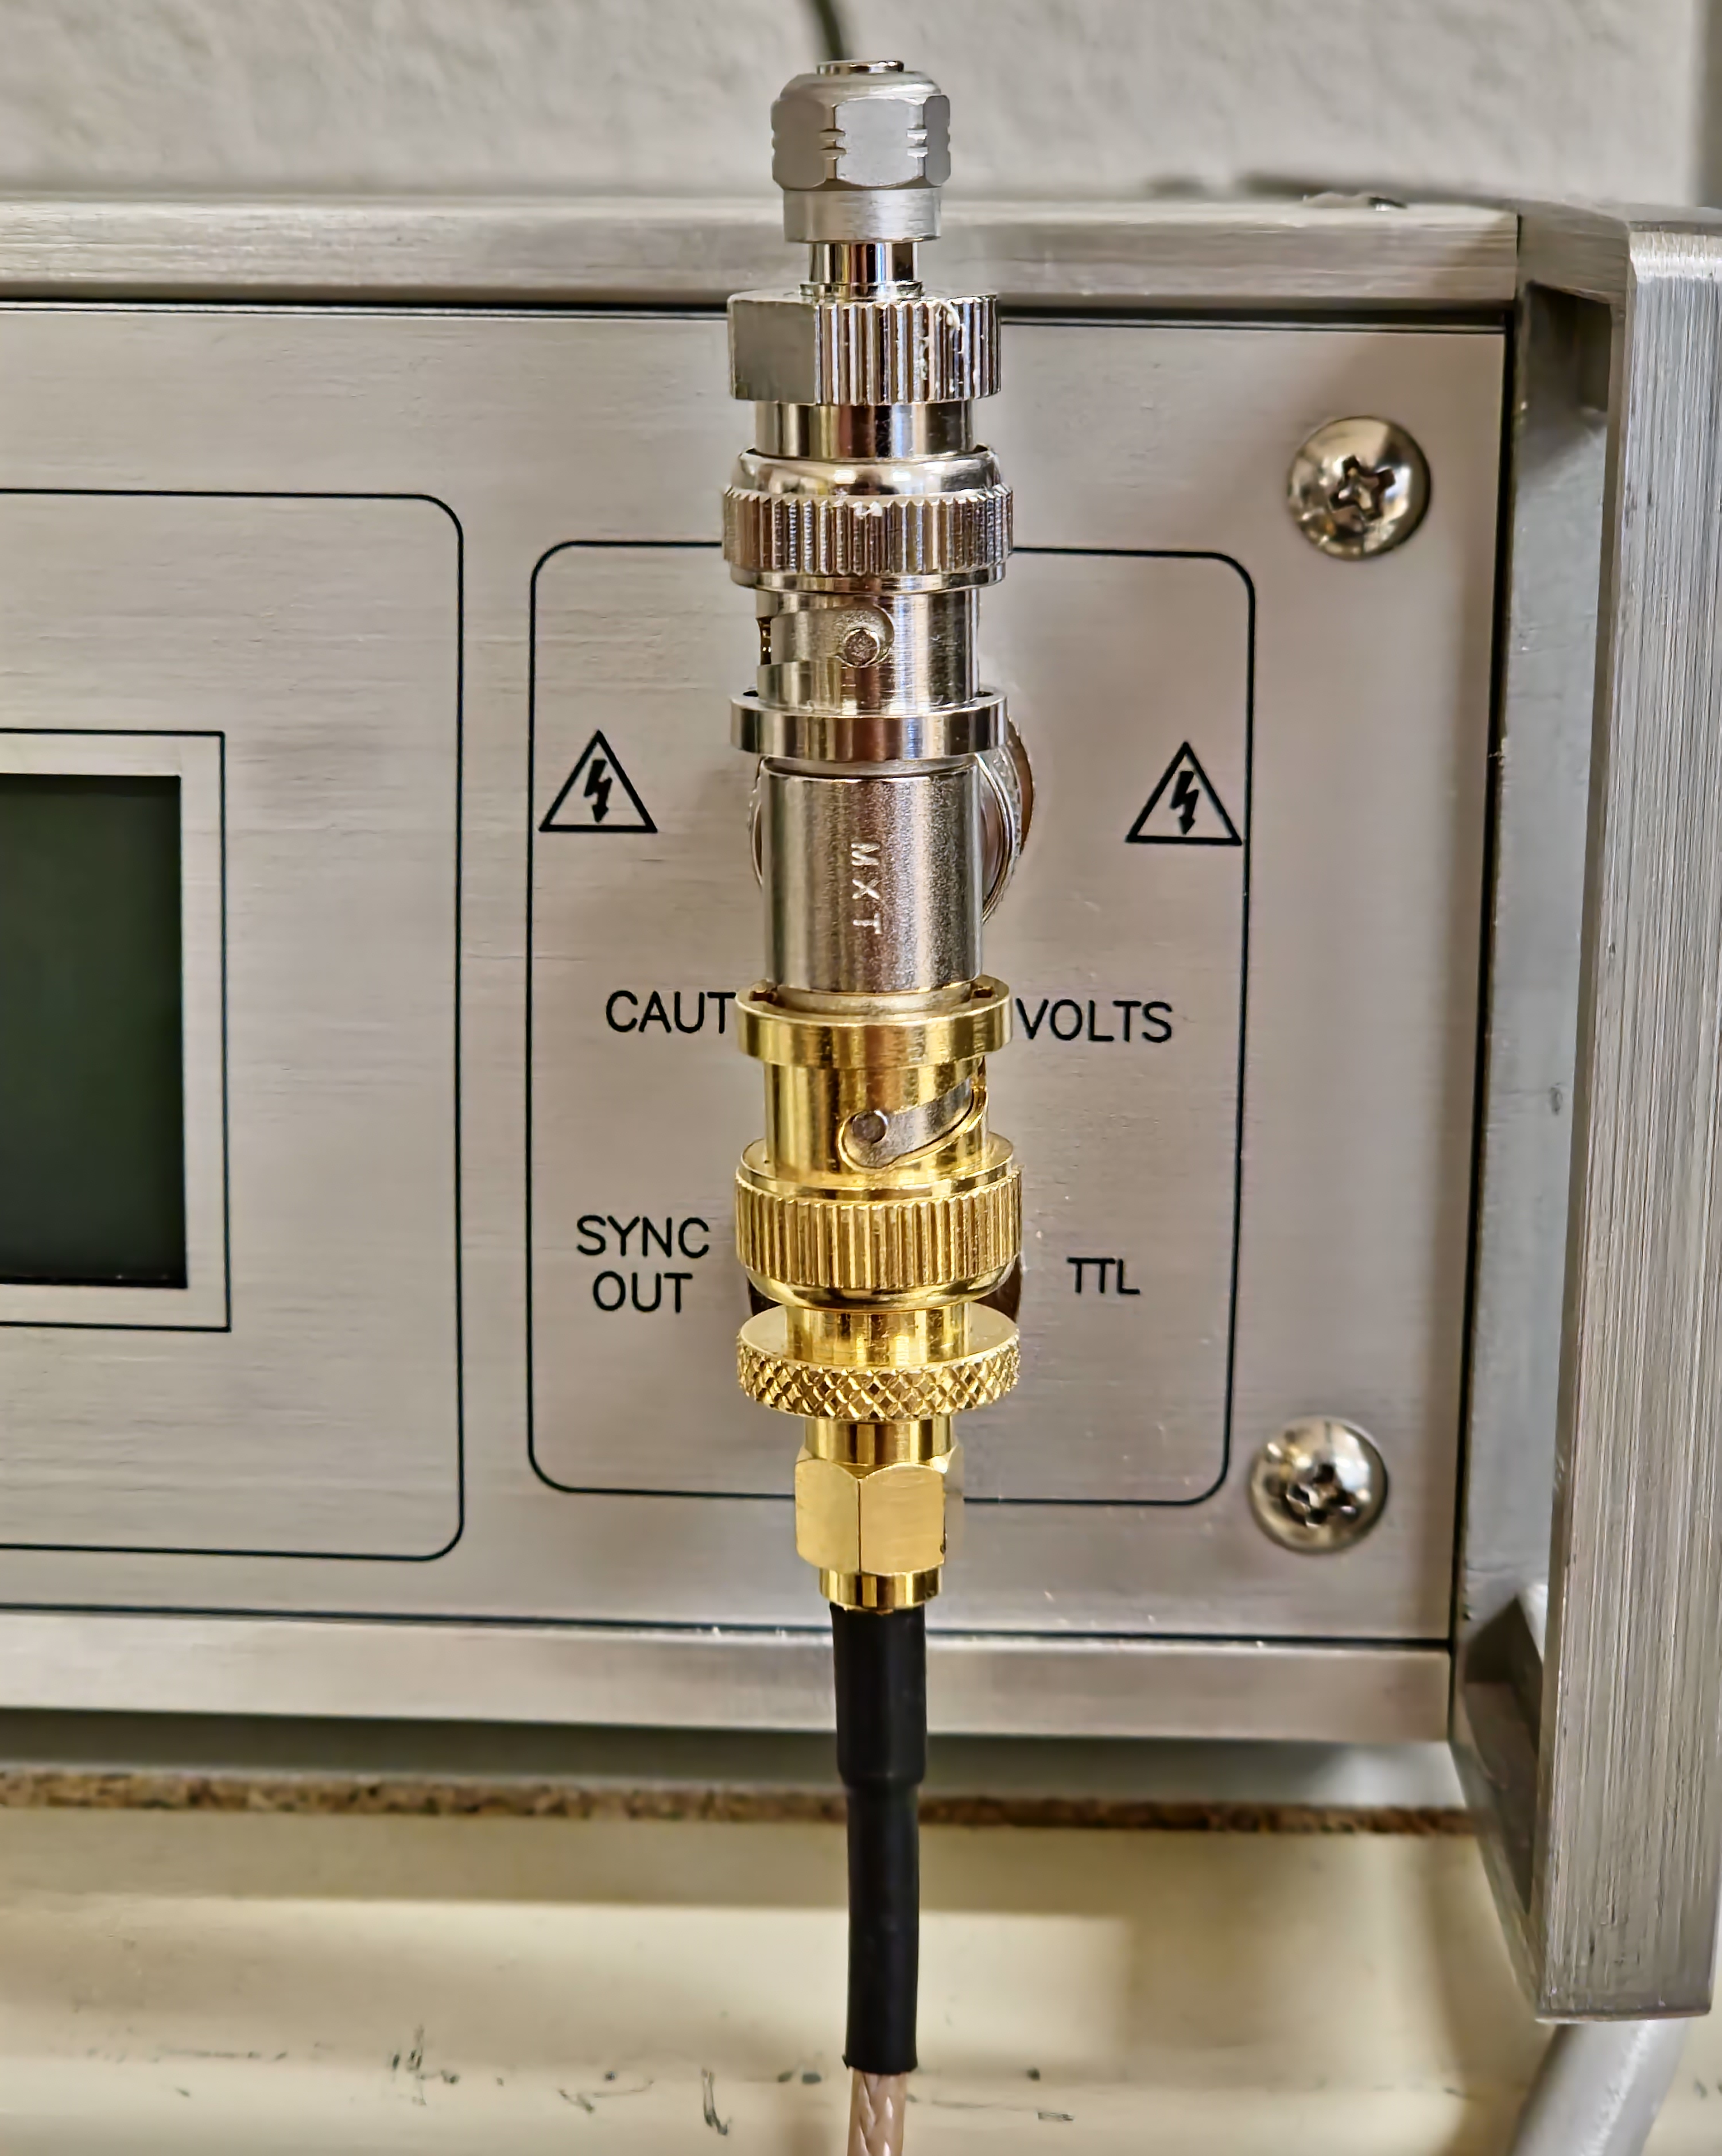
\includegraphics[width=0.3\textwidth, center]{2_goodPractices/figures/impMatchPicture.png}
%    \caption{Actual implementation of the proposed impedance matching.}
%    \label{fig:impMatchPhoto}
%\end{figure}


\begin{figure}[ht]
    \centering
%    \hfill
    \begin{subfigure}{0.48\textwidth}
        \centering
        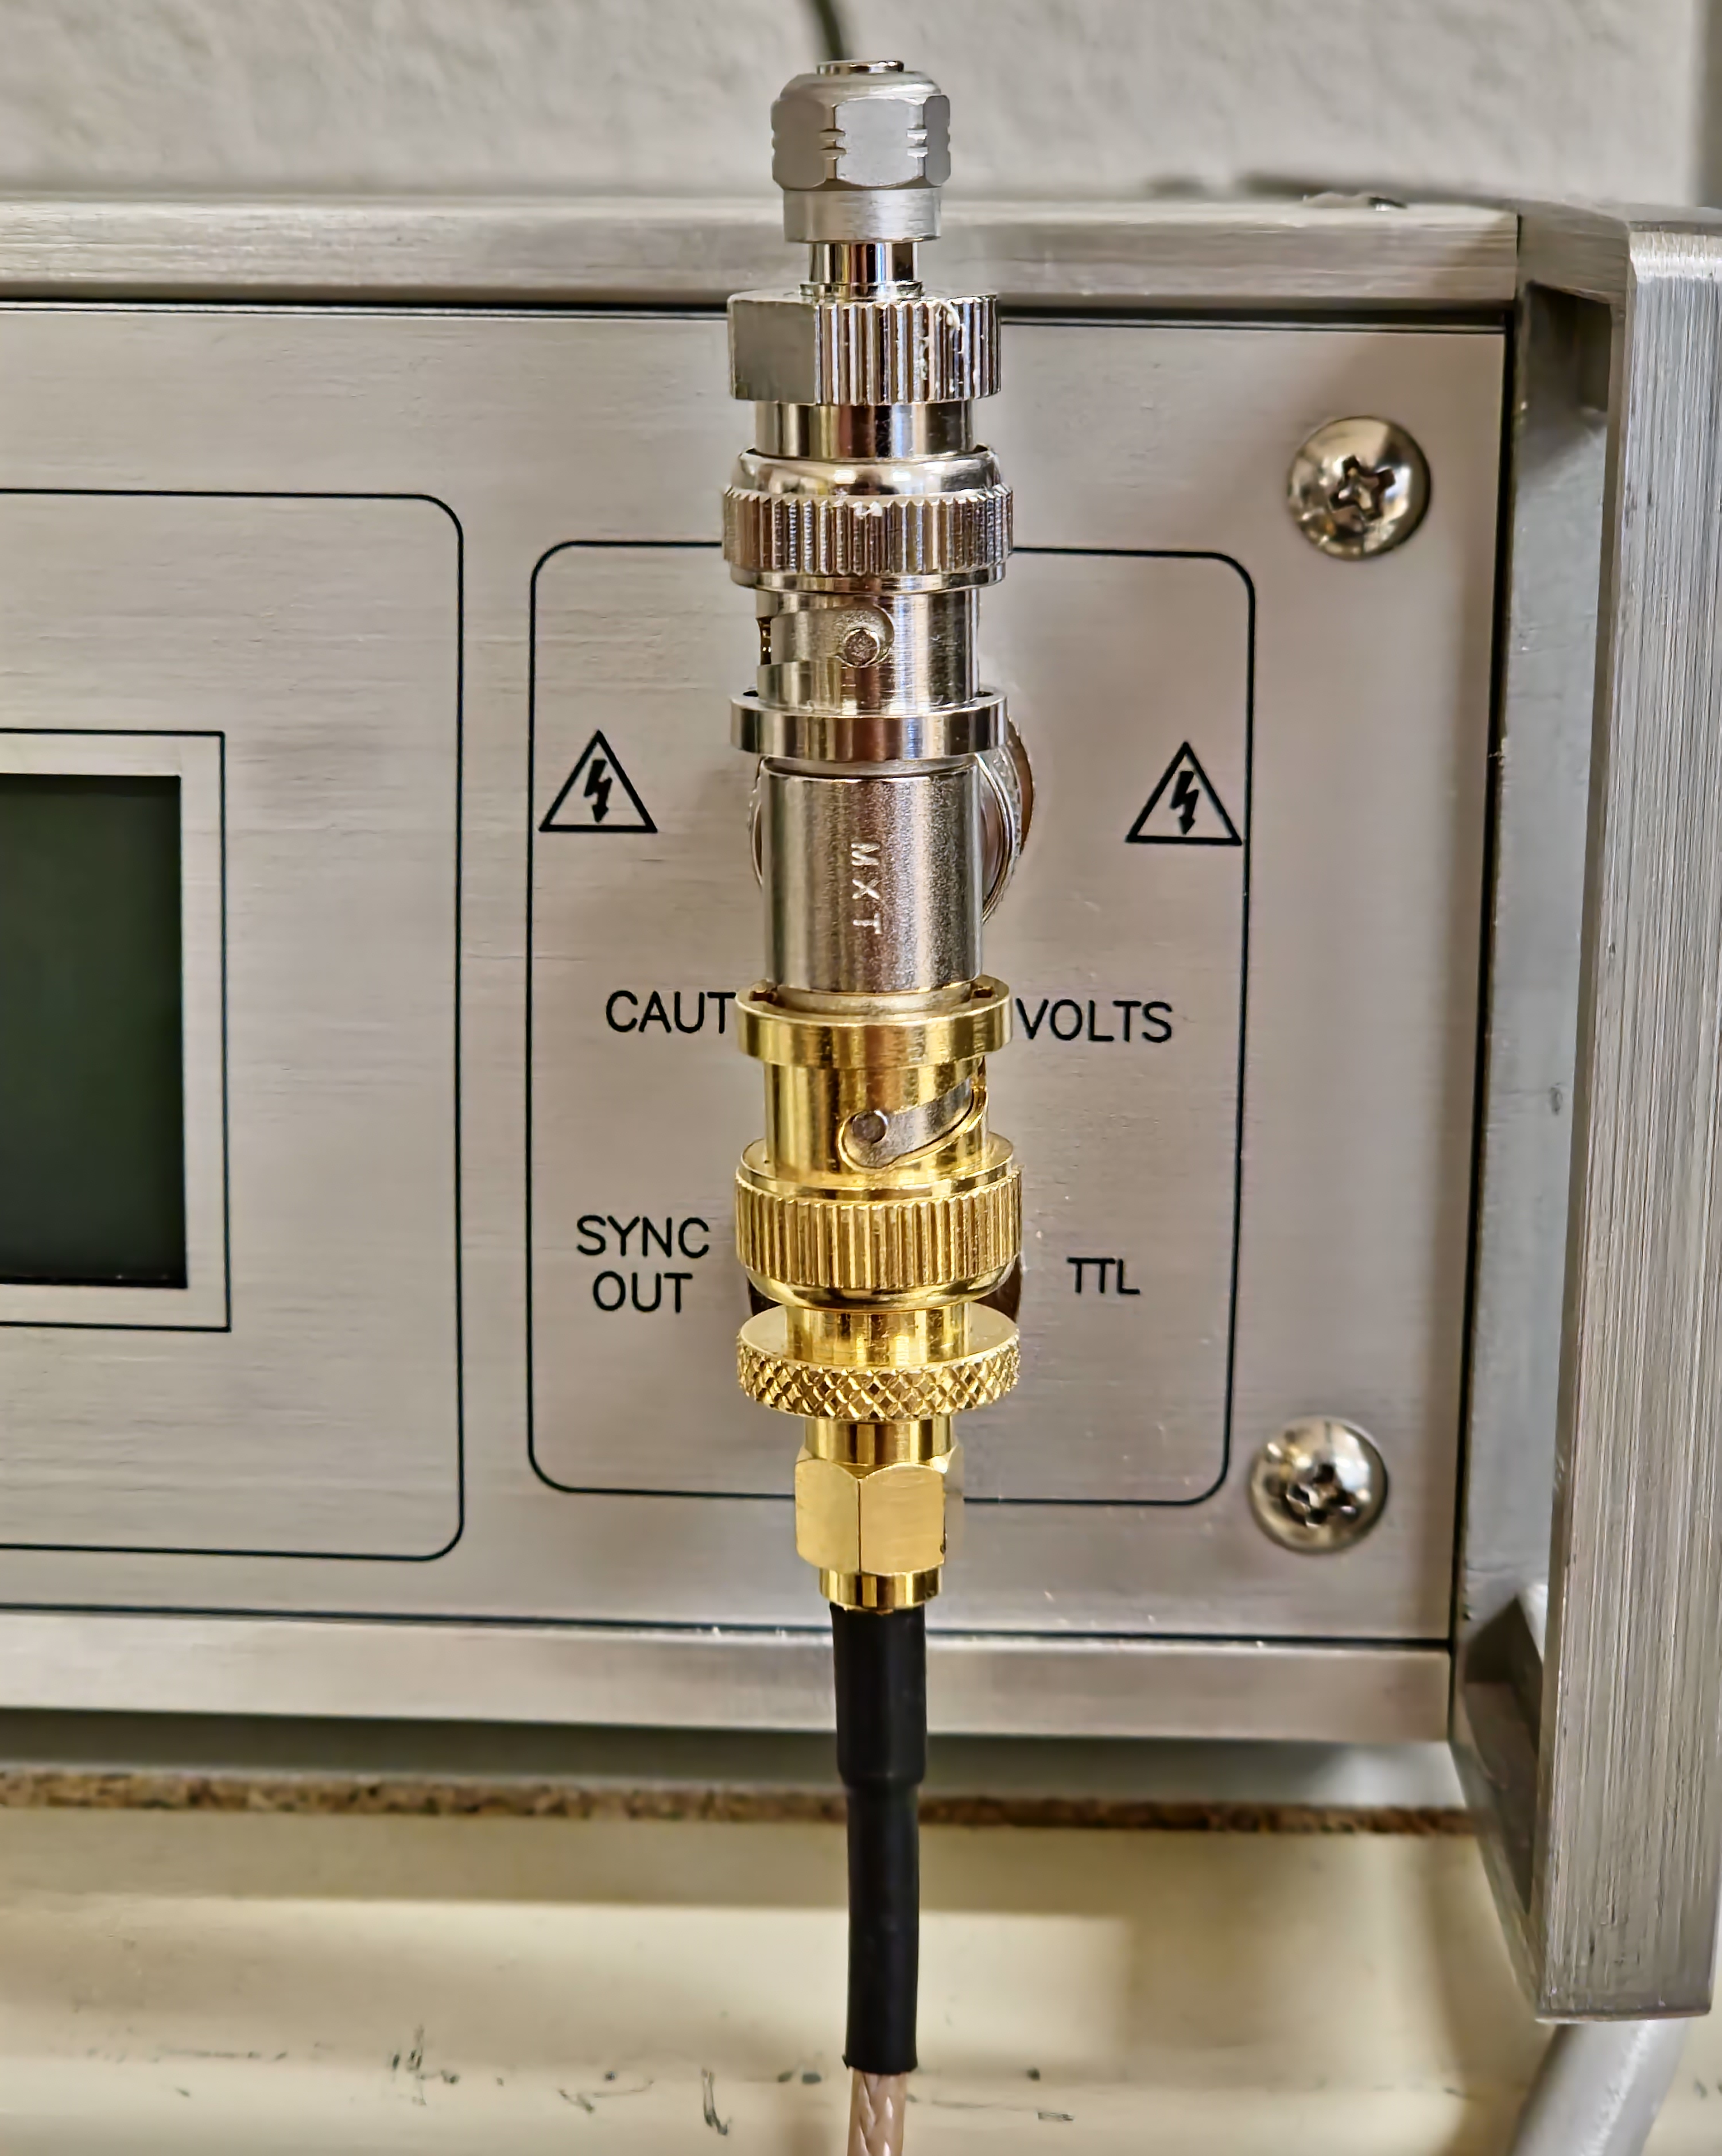
\includegraphics[width=0.60\textwidth, center]{2_goodPractices/figures/impMatchPicture.jpg}
        \caption{Actual implementation of the proposed impedance matching.}
        \label{fig:impMatchPhoto}
    \end{subfigure}
    \hfill
    \begin{subfigure}{0.48\textwidth}
        \centering
        \includegraphics[width=0.60\textwidth, center]{2_goodPractices/figures/sondeGndSource.jpg}
        \caption{Better alternative implementation of the impedance matching.}
        \label{fig:impMatchPhotoNew}
    \end{subfigure}
%    \hfill
    \caption{Actual pictures of a simple way to match the output impedance of the generator.}
    \label{fig:impMatch}
\end{figure}
